
\subsubsection{Duality}
\label{sec:duality}

\begin{prop}[UMP-EMP Duality]
  Suppose $u(x)$ is a continuous utility function satisfying local
  nonsatiation and $p >> 0$, then
  \begin{enumerate}[(a)]
  \item If $x^*$ is a solution to the UMP with wealth $w$, then $x^*$
    is a solution to the EMP with utility $u(x^*)$
  \item if $x^*$ is a solution to the EMP with utility $u_0$, then
    $x^*$ is a solution to the UMP with wealth $p \cdot x^*$.
  \end{enumerate}
\end{prop}


\subsubsection{Within UMP}
\label{sec:within-ump}

\begin{itemize}
\item We get $v(p,w) = u(x(p,w))$
\item We get $x(p,w)$ from $v(p,w)$ using Roy's Identity -- as long as
  $v$ is differentiable we get
  \[
  x_i(p^*, w^*)
  = - \frac{
    \frac{\partial v(p^*, w^*)}{\partial p_i}
  } {
    \frac{\partial v(p^*, w^*)}{\partial w}
  }
  \]
\end{itemize}

\subsubsection{From UMP to EMP}
\label{sec:from-ump-emp}

\begin{itemize}
\item We get $h(p, u) = x(p, e(p,u))$
\item We can get derivative information about $h$ from $x$ through the
  Slutsky Equation:
  \[
  \frac{\partial h_i (p, u_0)}{\partial p_j}
  = \frac{\partial x_i(p,w)}{\partial p_j}
  + \frac{\partial x_i(p,w)}{\partial w} x_j(p,w) 
  = s_{ij}
  \]
\item ** TODO ** can go $v \to e$ but MWG wrong
\end{itemize}


\subsubsection{Within EMP}
\label{sec:within-emp}

\begin{itemize}
\item We get $e(p,u) = p \cdot h(p,u)$
\item We get 
  \[
  h_i(p,u) = \frac{\partial}{\partial p_i} e(p,u)
  \]
\end{itemize}

\subsubsection{From EMP to UMP}
\label{sec:from-emp-ump}

\begin{itemize}
\item We get $x(p,w) = h(p, v(p,w))$
\item ** TODO ** can go $e \to v$ but MWG wrong
\item We can't go $h \to x$
\end{itemize}

\subsubsection{Summary}
\label{sec:eu-duality-summary}

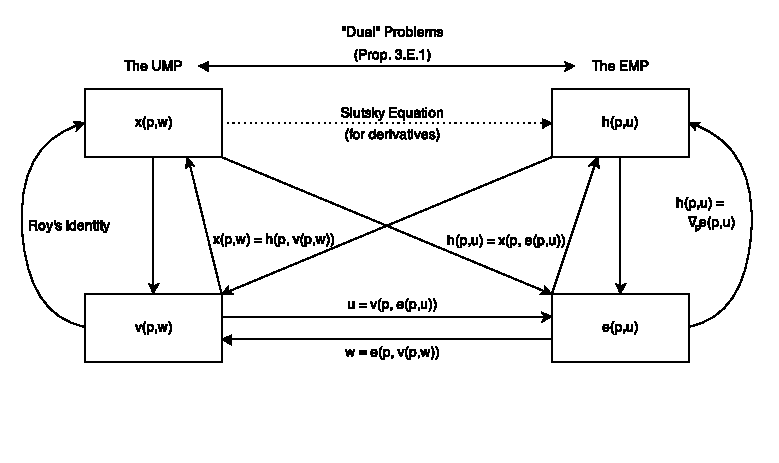
\includegraphics[width=0.9\textwidth]{./examnotes/mwg3d3.pdf}
%\includegraphics[width=0.9\textwidth]{./examnotes/dualityrelations}
